\documentclass[11pt,a4paper]{article}
\usepackage[utf8]{inputenc}
\usepackage[T1]{fontenc}
\usepackage{lmodern}
\usepackage[french]{babel}
\usepackage{amsmath,amssymb,amsthm,mathtools}
\usepackage[margin=2.4cm]{geometry}
\usepackage{xcolor}
\usepackage{graphicx}
\usepackage{tcolorbox}
\usepackage{tikz}
\usetikzlibrary{positioning,arrows.meta,calc}
\usepackage{hyperref}
\hypersetup{colorlinks=true,linkcolor=blue!50!black,citecolor=blue!50!black}

\numberwithin{equation}{section}
\setlength{\parindent}{0pt}
\setlength{\parskip}{4pt}

\theoremstyle{plain}
\newtheorem{theoreme}{Théorème}[section]
\newtheorem{lemme}[theoreme]{Lemme}
\newtheorem{proposition}[theoreme]{Proposition}
\theoremstyle{definition}
\newtheorem{definition}[theoreme]{Définition}
\newtheorem{hypothese}{Hypothèse}
\theoremstyle{remark}
\newtheorem{remarque}[theoreme]{Remarque}

\newcommand{\sign}{\operatorname{sign}}
\newcommand{\hth}{\hat{\theta}}
\newcommand{\hw}{\hat{\omega}}
\newcommand{\wff}{\omega_{ff}}
\newcommand{\sig}[1]{\lceil #1 \rfloor^{1/2}}

\newtcolorbox{idee}{colback=blue!4,colframe=blue!50!black,title=Idée,fonttitle=\bfseries}
\newtcolorbox{resultat}{colback=green!5,colframe=green!40!black,title=Résultat,fonttitle=\bfseries}
\newtcolorbox{attention}{colback=red!4,colframe=red!50!black,title=Attention,fonttitle=\bfseries}

\title{\textbf{Estimation de la position angulaire du réseau\\
par PLL à mode glissant d'ordre deux (Super-Twisting)}\\[4pt]
\large Développement complet : modélisation, dérivations et preuve de stabilité}
\date{}

\begin{document}
\maketitle
\tableofcontents
\newpage

%=====================================================================
\section{Objectif et vue d'ensemble}
%=====================================================================

On mesure les trois tensions du réseau $V_a,V_b,V_c$. On veut estimer en temps réel :
\begin{itemize}
  \item l'angle (la position) du réseau $\theta(t)$ ;
  \item la pulsation du réseau $\omega(t)=\dot\theta(t)$.
\end{itemize}
La chaîne de traitement est la suivante :
\[
(V_a,V_b,V_c)\xrightarrow{\text{Clarke}}(V_\alpha,V_\beta)
\xrightarrow{\text{Park avec }\hth}\varepsilon
\xrightarrow{\text{normalisation}}e
\xrightarrow{\text{Super-Twisting}}\hw
\xrightarrow{\int}\hth .
\]

\begin{figure}[h]
\centering
\begin{tikzpicture}[>=Stealth, node distance=1.0cm,
  blk/.style={draw,rounded corners,minimum height=9mm,minimum width=16mm,align=center,fill=blue!5},
  sum/.style={draw,circle,inner sep=1.5pt}]
\node (in) {$V_{abc}$};
\node[blk,right=0.6cm of in] (cl) {Clarke};
\node[blk,right=of cl] (pd) {Détecteur\\de phase\\ $\varepsilon/\hat V_m$};
\node[blk,right=of pd] (st) {Super-\\Twisting};
\node[sum,right=0.7cm of st] (s) {$+$};
\node[blk,right=0.7cm of s] (int) {$\displaystyle\int$};
\node[right=0.6cm of int] (out) {$\hth$};
\node[above=0.6cm of s] (ff) {$\wff$};
\draw[->] (in)--(cl);
\draw[->] (cl)--node[above]{$V_{\alpha\beta}$}(pd);
\draw[->] (pd)--node[above]{$e$}(st);
\draw[->] (st)--(s);
\draw[->] (ff)--(s);
\draw[->] (s)--node[above]{$\hw$}(int);
\draw[->] (int)--(out);
\draw[->] ($(int.east)+(0.3,0)$)--++(0,-1.2)-|node[pos=0.25,below]{$\hth$}(pd.south);
\end{tikzpicture}
\caption{Structure de la PLL Super-Twisting.}
\end{figure}

Le document suit cette chaîne bloc par bloc. Chaque calcul est développé ligne par ligne.
L'annexe~\ref{sec:annexe} rassemble toutes les formules mathématiques utilisées.

%=====================================================================
\section{Modèle des tensions du réseau}
%=====================================================================

\subsection{Angle et pulsation}
\begin{definition}
L'angle du réseau est l'intégrale de la pulsation :
\begin{equation}\label{eq:theta}
\theta(t) = \theta_0 + \int_0^t \omega(\tau)\,d\tau
\qquad\Longleftrightarrow\qquad
\boxed{\dot\theta(t) = \omega(t).}
\end{equation}
Si la fréquence est constante, $\omega(t)=\omega$ et on retrouve $\theta(t)=\omega t+\theta_0$.
\end{definition}

\subsection{Tensions triphasées équilibrées}
On adopte la convention \textbf{cosinus} :
\begin{align}
V_a &= V_m\cos\theta, \label{eq:va}\\
V_b &= V_m\cos\!\left(\theta-\tfrac{2\pi}{3}\right), \label{eq:vb}\\
V_c &= V_m\cos\!\left(\theta+\tfrac{2\pi}{3}\right). \label{eq:vc}
\end{align}
\begin{remarque}
On a $\theta-\tfrac{4\pi}{3} = \theta+\tfrac{2\pi}{3}-2\pi$. Comme le cosinus est $2\pi$-périodique,
$\cos(\theta-\tfrac{4\pi}{3})=\cos(\theta+\tfrac{2\pi}{3})$. Les deux écritures de $V_c$ sont donc équivalentes.
\end{remarque}

\subsection{Somme des trois tensions}
\begin{lemme}\label{lem:somme}
$V_a+V_b+V_c = 0$.
\end{lemme}
\begin{proof}
On utilise la formule \eqref{A:sum} de l'annexe, $\cos(a-b)+\cos(a+b)=2\cos a\cos b$,
avec $a=\theta$ et $b=\tfrac{2\pi}{3}$ :
\begin{align}
V_b+V_c &= V_m\left[\cos\!\left(\theta-\tfrac{2\pi}{3}\right)+\cos\!\left(\theta+\tfrac{2\pi}{3}\right)\right]\\
&= V_m\cdot 2\cos\theta\cos\tfrac{2\pi}{3}.
\end{align}
Or $\cos\tfrac{2\pi}{3} = -\tfrac12$, donc
\begin{equation}\label{eq:vbpvc}
V_b+V_c = V_m\cdot 2\cos\theta\cdot\left(-\tfrac12\right) = -V_m\cos\theta = -V_a .
\end{equation}
D'où $V_a+V_b+V_c = V_a - V_a = 0$.
\end{proof}

%=====================================================================
\section{Transformation de Clarke}
%=====================================================================

\subsection{Définition}
La transformation de Clarke (version \emph{invariante en amplitude}, facteur $2/3$) s'écrit
\begin{align}
V_\alpha &= \frac23\left(V_a-\frac12V_b-\frac12V_c\right), \label{eq:clarke_a}\\
V_\beta  &= \frac23\left(\frac{\sqrt3}{2}V_b-\frac{\sqrt3}{2}V_c\right). \label{eq:clarke_b}
\end{align}
Sous forme matricielle :
\begin{equation}
\begin{bmatrix}V_\alpha\\V_\beta\end{bmatrix}
=\frac23\begin{bmatrix}1&-\tfrac12&-\tfrac12\\[2pt]0&\tfrac{\sqrt3}{2}&-\tfrac{\sqrt3}{2}\end{bmatrix}
\begin{bmatrix}V_a\\V_b\\V_c\end{bmatrix}.
\end{equation}

\subsection{Calcul de $V_\alpha$}
\textbf{Étape 1.} On factorise $-\frac12$ :
\begin{equation}
V_\alpha = \frac23\left(V_a-\frac12\,(V_b+V_c)\right).
\end{equation}
\textbf{Étape 2.} On utilise \eqref{eq:vbpvc}, $V_b+V_c=-V_m\cos\theta$ :
\begin{equation}
V_\alpha = \frac23\left(V_m\cos\theta+\frac12V_m\cos\theta\right) = \frac23\cdot\frac32\,V_m\cos\theta .
\end{equation}
\textbf{Étape 3.}
\begin{equation}\label{eq:valpha}
\boxed{V_\alpha = V_m\cos\theta.}
\end{equation}

\subsection{Calcul de $V_\beta$}
\textbf{Étape 1.} On factorise $\frac{\sqrt3}{2}$ :
\begin{equation}
V_\beta = \frac23\cdot\frac{\sqrt3}{2}\,(V_b-V_c) = \frac{1}{\sqrt3}\,(V_b-V_c).
\end{equation}
\textbf{Étape 2.} On utilise la formule \eqref{A:diff}, $\cos(a-b)-\cos(a+b) = 2\sin a\sin b$,
avec $a=\theta$ et $b=\tfrac{2\pi}{3}$ :
\begin{equation}
V_b-V_c = V_m\left[\cos\!\left(\theta-\tfrac{2\pi}{3}\right)-\cos\!\left(\theta+\tfrac{2\pi}{3}\right)\right]
= 2V_m\sin\theta\sin\tfrac{2\pi}{3}.
\end{equation}
\textbf{Étape 3.} Comme $\sin\tfrac{2\pi}{3}=\tfrac{\sqrt3}{2}$ :
\begin{equation}
V_b-V_c = 2V_m\sin\theta\cdot\tfrac{\sqrt3}{2} = \sqrt3\,V_m\sin\theta .
\end{equation}
\textbf{Étape 4.}
\begin{equation}\label{eq:vbeta}
V_\beta = \frac{1}{\sqrt3}\cdot\sqrt3\,V_m\sin\theta \quad\Longrightarrow\quad \boxed{V_\beta = V_m\sin\theta.}
\end{equation}

\subsection{Interprétation}\label{sec:conv}
Le vecteur $(V_\alpha,V_\beta) = V_m(\cos\theta,\sin\theta)$ est un vecteur de longueur $V_m$
qui tourne dans le plan à la vitesse $\omega$. Son angle polaire est exactement $\theta$.
Estimer la position du réseau revient donc à estimer l'angle de ce vecteur tournant.

\begin{attention}
\textbf{Convention sinus.} Si l'on écrit $V_a=V_m\sin\theta$, $V_b=V_m\sin(\theta-\frac{2\pi}{3})$
et $V_c=V_m\sin(\theta+\frac{2\pi}{3})$, le même calcul donne
\[
V_\alpha = V_m\sin\theta,\qquad V_\beta = -V_m\cos\theta .
\]
\emph{Démonstration :} $\sin\theta = \cos(\theta-\frac{\pi}{2})$. Le calcul précédent, appliqué à
$\theta'=\theta-\frac\pi2$, donne $V_\alpha=V_m\cos\theta'=V_m\sin\theta$ et
$V_\beta=V_m\sin\theta'=V_m\sin(\theta-\frac\pi2)=-V_m\cos\theta$.

La PLL estime alors $\theta' = \theta-\pi/2$ et non $\theta$. Au tableau, les deux conventions étaient
mélangées : $V_a=V_m\sin\theta$, mais $V_\alpha=V_m\cos\theta$. Il faut en choisir \textbf{une seule}.
\end{attention}

\subsection{Pourquoi le facteur $2/3$ ?}
Sans le facteur $2/3$, on obtiendrait $V_\alpha = \frac32V_m\cos\theta$. Le facteur $2/3$ rend
l'amplitude du vecteur $(V_\alpha,V_\beta)$ égale à l'amplitude $V_m$ d'une phase.
C'est la version dite \og invariante en amplitude\fg.

%=====================================================================
\section{Détecteur de phase (transformation de Park)}
%=====================================================================

\subsection{Rotation par l'angle estimé}
Soit $\hth$ l'angle estimé par la PLL. On fait tourner le vecteur $(V_\alpha,V_\beta)$ de $-\hth$
(transformation de Park) :
\begin{equation}
\begin{bmatrix}V_d\\V_q\end{bmatrix}
=\begin{bmatrix}\cos\hth&\sin\hth\\-\sin\hth&\cos\hth\end{bmatrix}
\begin{bmatrix}V_\alpha\\V_\beta\end{bmatrix}.
\end{equation}

\subsection{Calcul de $V_q$}
\textbf{Étape 1.} On lit la deuxième ligne de la matrice :
\begin{equation}
V_q = -V_\alpha\sin\hth + V_\beta\cos\hth .
\end{equation}
\textbf{Étape 2.} On remplace par \eqref{eq:valpha} et \eqref{eq:vbeta} :
\begin{equation}
V_q = -V_m\cos\theta\sin\hth + V_m\sin\theta\cos\hth
    = V_m\big[\sin\theta\cos\hth-\cos\theta\sin\hth\big].
\end{equation}
\textbf{Étape 3.} On reconnaît la formule \eqref{A:sin}, $\sin(a-b)=\sin a\cos b-\cos a\sin b$ :
\begin{equation}\label{eq:eps}
\boxed{\varepsilon \triangleq V_q = V_m\sin(\theta-\hth).}
\end{equation}

\subsection{Calcul de $V_d$ (pour information)}
\begin{equation}
V_d = V_\alpha\cos\hth + V_\beta\sin\hth = V_m[\cos\theta\cos\hth+\sin\theta\sin\hth] = V_m\cos(\theta-\hth).
\end{equation}
Quand la PLL est verrouillée ($\hth=\theta$), on a $V_d=V_m$ et $V_q=0$.

\subsection{Erreur de phase}
\begin{definition}
L'erreur de phase est
\begin{equation}\label{eq:psi}
\boxed{\psi \triangleq \theta-\hth .}
\end{equation}
Le signal du détecteur s'écrit donc $\varepsilon = V_m\sin\psi$.
\end{definition}

\subsection{Propriétés du détecteur}
\begin{itemize}
  \item $\varepsilon=0$ si et seulement si $\psi=0$ ou $\psi=\pi$ (modulo $2\pi$).
  \item Pour $\psi$ petit : $\sin\psi\approx\psi$, donc $\varepsilon\approx V_m\psi$. Le détecteur est
        alors \emph{linéaire}, avec un gain $V_m$.
  \item Pour $0<|\psi|<\pi$ : $\sign(\varepsilon) = \sign(\psi)$ (démontré au lemme~\ref{lem:signe}).
        Le signe de $\varepsilon$ indique donc si l'estimation est en retard ($\psi>0$) ou en avance ($\psi<0$).
\end{itemize}

\begin{figure}[h]
\centering
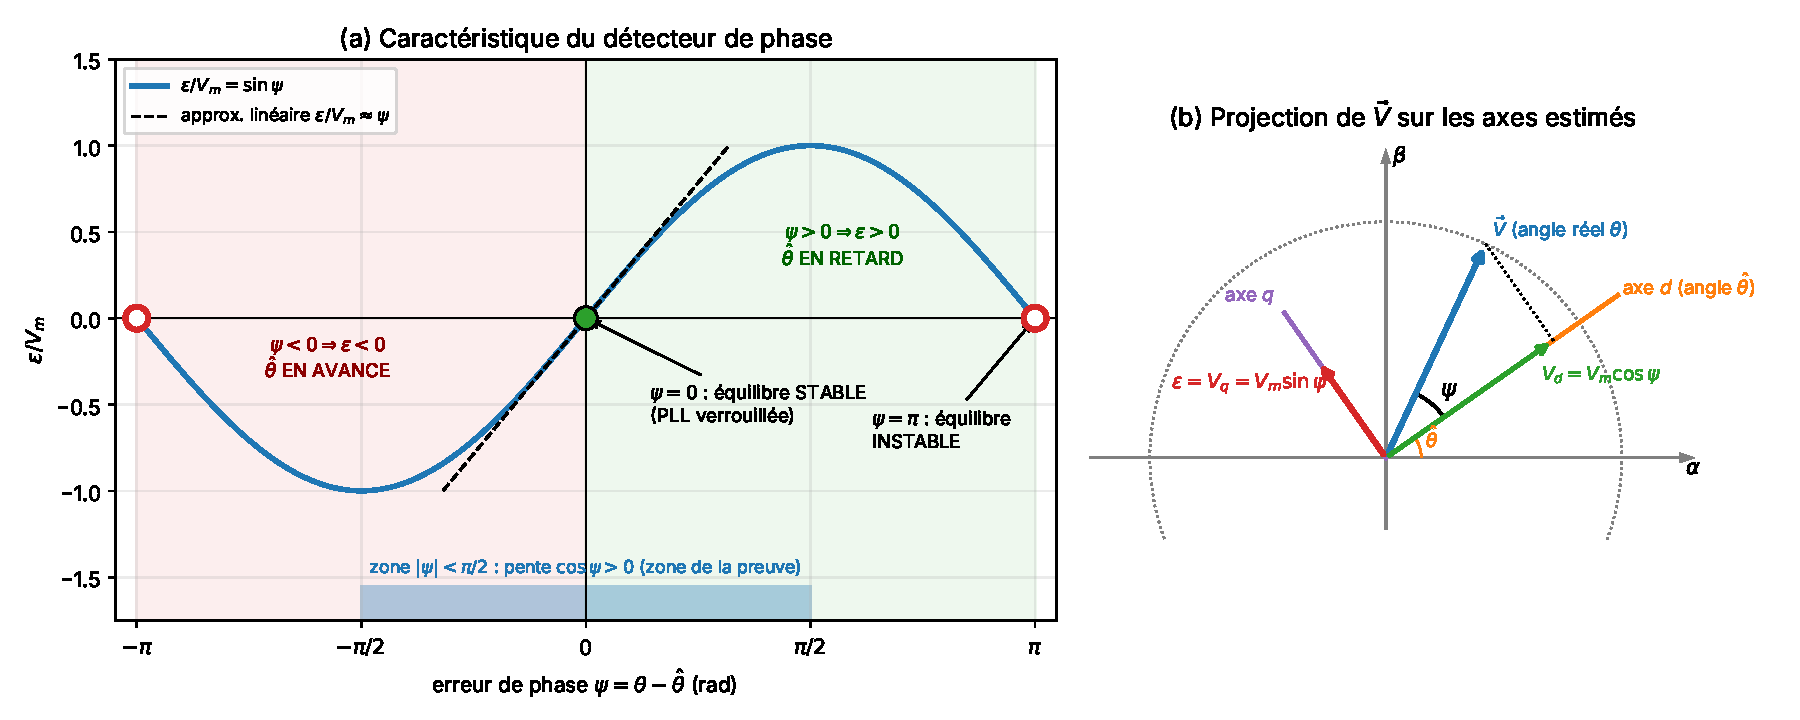
\includegraphics[width=\textwidth]{figures/detecteur_phase.pdf}
\caption{(a) Caractéristique $\varepsilon/V_m=\sin\psi$ : zéros en $\psi=0$ (stable) et $\psi=\pi$ (instable),
zone linéaire autour de $0$, et signe de $\varepsilon$ qui indique le retard ou l'avance.
(b) Interprétation géométrique : $\varepsilon$ est la projection du vecteur tournant $\vec V$ sur l'axe $q$ estimé.}
\end{figure}

\subsection{Normalisation par l'amplitude}
\textbf{Étape 1.} On calcule l'amplitude du vecteur $\alpha\beta$ :
\begin{equation}
V_\alpha^2+V_\beta^2 = V_m^2\cos^2\theta+V_m^2\sin^2\theta = V_m^2(\cos^2\theta+\sin^2\theta) = V_m^2 .
\end{equation}
\textbf{Étape 2.} On en déduit l'estimation de l'amplitude :
\begin{equation}
\hat V_m = \sqrt{V_\alpha^2+V_\beta^2} = V_m .
\end{equation}
\textbf{Étape 3.} On définit l'erreur normalisée :
\begin{equation}\label{eq:e}
\boxed{e \triangleq \frac{\varepsilon}{\hat V_m} = \frac{-V_\alpha\sin\hth+V_\beta\cos\hth}{\sqrt{V_\alpha^2+V_\beta^2}} = \sin\psi .}
\end{equation}
\begin{idee}
Grâce à la normalisation, $e$ ne dépend plus de $V_m$ et reste toujours dans $[-1,1]$.
Les gains de la PLL n'ont donc pas à être recalculés si l'amplitude du réseau change (creux de tension).
\end{idee}

%=====================================================================
\section{Dynamique de l'erreur de phase}
%=====================================================================

\subsection{Loi de l'intégrateur}
L'angle estimé est l'intégrale de la pulsation estimée :
\begin{equation}\label{eq:thetahat}
\dot\hth = \hw .
\end{equation}

\subsection{Dérivée de $\psi$}
\textbf{Étape 1.} On dérive la définition \eqref{eq:psi} :
\begin{equation}
\dot\psi = \frac{d}{dt}(\theta-\hth) = \dot\theta-\dot\hth .
\end{equation}
\textbf{Étape 2.} On remplace par \eqref{eq:theta} et \eqref{eq:thetahat} :
\begin{equation}\label{eq:psidot}
\boxed{\dot\psi = \omega-\hw .}
\end{equation}

\subsection{Dérivée de $e$ et de $\varepsilon$}\label{sec:edot}
$e=\sin\psi$ est une fonction composée : la fonction $\sin$ appliquée à $\psi(t)$.
On applique la règle de dérivation en chaîne \eqref{A:chain} :
\begin{equation}
\dot e = \frac{de}{d\psi}\cdot\frac{d\psi}{dt} = \cos\psi\cdot\dot\psi = \cos\psi\,(\omega-\hw).
\end{equation}
Si $V_m$ est constant, $\varepsilon = V_m\sin\psi$ et
\begin{equation}
\dot\varepsilon = V_m\cos\psi\,\dot\psi = V_m\cos\psi\,(\omega-\hw).
\end{equation}
Si $V_m$ varie, on applique la règle du produit \eqref{A:prod} :
\begin{equation}
\dot\varepsilon = \dot V_m\sin\psi + V_m\cos\psi\,\dot\psi .
\end{equation}
Le premier terme est une perturbation. La normalisation \eqref{eq:e} l'élimine.

\begin{attention}
Au tableau, on avait écrit $\dot\varepsilon = V_m\cos\psi$. C'est en réalité la dérivée par rapport
à l'angle, $\partial\varepsilon/\partial\theta = V_m\cos\psi$ (le gain du détecteur), et non la dérivée
par rapport au temps. Il manque le facteur $\dot\psi$.

Vérification avec les dérivées partielles :
\[
\dot\varepsilon = \frac{\partial\varepsilon}{\partial\theta}\dot\theta + \frac{\partial\varepsilon}{\partial\hth}\dot\hth
= V_m\cos\psi\cdot\omega + (-V_m\cos\psi)\cdot\hw = V_m\cos\psi(\omega-\hw).
\]
\end{attention}

%=====================================================================
\section{Choix de la loi d'estimation}
%=====================================================================

\subsection{Quel signe ? Étude d'une loi proportionnelle}\label{sec:signe}
On essaie d'abord la loi la plus simple :
\begin{equation}
\hw = k\,e + \wff = k\sin\psi + \wff,\qquad k>0 .
\end{equation}
On suppose d'abord $\omega=\wff$ (fréquence nominale). Alors
\begin{equation}
\dot\psi = \omega-\hw = \wff - k\sin\psi - \wff = -k\sin\psi .
\end{equation}
On prend $V_0=\frac12\psi^2$. Sa dérivée est
\begin{equation}
\dot V_0 = \psi\dot\psi = -k\,\psi\sin\psi .
\end{equation}
Pour $0<|\psi|<\pi$, $\psi$ et $\sin\psi$ ont le même signe, donc $\psi\sin\psi>0$ et $\dot V_0<0$.
L'erreur décroît.

\begin{resultat}
Le gain doit être \textbf{positif} devant $e$ dans la loi sur $\hw$. Avec un signe négatif,
$\dot V_0 = +k\psi\sin\psi>0$ et l'erreur augmente : l'estimateur diverge.
\end{resultat}

\textbf{Explication physique.} Si $\psi>0$, l'estimation $\hth$ est en retard sur $\theta$.
Il faut que $\hth$ tourne plus vite, donc il faut augmenter $\hw$.

\subsection{Limite de la loi proportionnelle}
Si $\omega\neq\wff$, on cherche l'équilibre $\dot\psi=0$ :
\begin{equation}
0 = \omega - k\sin\psi^\star-\wff \quad\Longrightarrow\quad \sin\psi^\star = \frac{\omega-\wff}{k}.
\end{equation}
L'erreur statique $\psi^\star$ n'est pas nulle. Il faut un intégrateur.

\subsection{Limite de la loi PI}\label{sec:pi}
Avec $\hw = k_pe + z + \wff$ et $\dot z = k_ie$, on considère une rampe de fréquence
$\omega = \omega_0 + at$. En régime établi, $\psi$ est constant, donc $\dot\psi=0$, $\hw=\omega$
et $\dot\hw = a$. Or
\begin{equation}
\dot\hw = k_p\dot e + \dot z = k_p\cdot 0 + k_ie \quad\Longrightarrow\quad e^\star = \sin\psi^\star = \frac{a}{k_i}\neq 0 .
\end{equation}
La PLL PI garde donc une erreur de phase pendant une rampe de fréquence.

\subsection{Loi Super-Twisting}
\begin{definition}
La loi d'estimation Super-Twisting est
\begin{align}
\hw &= k_1\,|e|^{1/2}\sign(e) + z + \wff, \label{eq:st1}\\
\dot z &= k_2\,\sign(e), \label{eq:st2}\\
\dot\hth &= \hw , \label{eq:st3}
\end{align}
avec $k_1>0$, $k_2>0$ et $\wff$ une constante (par exemple $2\pi\cdot50$ rad/s).
\end{definition}

\textbf{Rôle de chaque terme :}
\begin{itemize}
  \item $k_1|e|^{1/2}\sign(e)$ : terme \og proportionnel\fg{} non linéaire. La puissance $1/2$ rend ce
        terme plus fort qu'un terme linéaire quand $e$ est petit (car $|e|^{1/2}>|e|$ pour $|e|<1$).
        C'est ce qui donne la convergence en \emph{temps fini}.
  \item $z$ : terme \og intégral\fg. Il apprend l'écart de fréquence $\omega-\wff$.
  \item $\sign(e)$ dans $\dot z$ : la discontinuité est \emph{intégrée}, donc $z$ et $\hw$ restent
        \textbf{continus}. Il n'y a pas de broutement (chattering) sur la fréquence estimée.
  \item $\wff$ : anticipation (feed-forward) de la fréquence nominale.
\end{itemize}
Tous les signes sont \og $+$\fg, conformément à la section~\ref{sec:signe}.

\begin{attention}
Au tableau, la loi était écrite
$\hw = -k_1|\varepsilon|^{1/2}\sign(\varepsilon)+z$, $\dot z=-k_2\sign(\varepsilon)$.
C'est la forme canonique du Super-Twisting, mais cette forme décrit la dynamique \emph{de l'erreur}
(section~\ref{sec:chgt}), et non la loi d'estimation. Avec ces signes, la PLL diverge.
\end{attention}

%=====================================================================
\section{Changement de variables : équations de l'erreur}\label{sec:chgt}
%=====================================================================

\subsection{Pourquoi changer de variables ?}
\begin{idee}
L'implémentation utilise $\hth$ et $z$. Pour étudier la stabilité, on veut des variables qui valent
$0$ quand la PLL est parfaitement verrouillée. On montrera ensuite qu'elles tendent vers $0$.
\end{idee}

\subsection{Choix de $x_1$}
On veut $\hth=\theta$, donc on pose
\begin{equation}
\boxed{x_1 \triangleq \psi = \theta-\hth .}
\end{equation}

\subsection{Choix de $x_2$}
\textbf{Étape 1.} Quand la PLL est verrouillée, $\hw=\omega$ et $e=0$. On remplace dans \eqref{eq:st1} :
\begin{equation}
\omega = k_1\cdot 0 + z + \wff \quad\Longrightarrow\quad z = \omega-\wff .
\end{equation}
\textbf{Étape 2.} L'intégrateur doit donc converger vers $\omega-\wff$. On mesure ce qui lui manque :
\begin{equation}
\boxed{x_2 \triangleq (\omega-\wff)-z .}
\end{equation}

\begin{center}
\begin{tabular}{lcc}
\hline
 & PLL verrouillée & PLL non verrouillée\\
\hline
$x_1=\theta-\hth$ & $0$ & $\neq0$\\
$x_2=(\omega-\wff)-z$ & $0$ & $\neq0$\\
\hline
\end{tabular}
\end{center}

\subsection{Signe du sinus}
\begin{lemme}\label{lem:signe}
Pour $|x|<\pi$ : $\sign(\sin x)=\sign(x)$.
\end{lemme}
\begin{proof}
On distingue trois cas.
\begin{itemize}
  \item Si $0<x<\pi$, alors $\sin x>0$, donc $\sign(\sin x)=+1=\sign(x)$.
  \item Si $-\pi<x<0$, alors $\sin x = -\sin(-x)$ avec $0<-x<\pi$, donc $\sin x<0$ et $\sign(\sin x)=-1=\sign(x)$.
  \item Si $x=0$, alors $\sin 0=0$ et $\sign(0)=0$.
\end{itemize}
\end{proof}

\subsection{Calcul de $\dot x_1$}
\textbf{Étape 1.} D'après \eqref{eq:psidot} :
\begin{equation}
\dot x_1 = \omega-\hw .
\end{equation}
\textbf{Étape 2.} On remplace $\hw$ par \eqref{eq:st1} :
\begin{equation}
\dot x_1 = \omega - k_1|e|^{1/2}\sign(e) - z - \wff .
\end{equation}
\textbf{Étape 3.} On regroupe $\omega$, $\wff$ et $z$ :
\begin{equation}
\dot x_1 = -k_1|e|^{1/2}\sign(e) + \underbrace{(\omega-\wff)-z}_{=\,x_2}
        = -k_1|e|^{1/2}\sign(e) + x_2 .
\end{equation}
\textbf{Étape 4.} On remplace $e=\sin x_1$ et on applique le lemme~\ref{lem:signe} :
\begin{equation}\label{eq:x1dot}
\boxed{\dot x_1 = -k_1|\sin x_1|^{1/2}\sign(x_1) + x_2 .}
\end{equation}

\subsection{Calcul de $\dot x_2$}
\textbf{Étape 1.} On dérive la définition de $x_2$ :
\begin{equation}
\dot x_2 = \dot\omega - \dot\omega_{ff} - \dot z .
\end{equation}
\textbf{Étape 2.} $\wff$ est constante, donc $\dot\omega_{ff}=0$. On remplace $\dot z$ par \eqref{eq:st2} :
\begin{equation}
\dot x_2 = \dot\omega - k_2\sign(e) .
\end{equation}
\textbf{Étape 3.} On applique encore $\sign(e)=\sign(\sin x_1)=\sign(x_1)$ :
\begin{equation}\label{eq:x2dot}
\boxed{\dot x_2 = -k_2\sign(x_1) + \dot\omega(t) .}
\end{equation}

\subsection{Récapitulatif des substitutions}
\begin{center}
\renewcommand{\arraystretch}{1.3}
\begin{tabular}{|l|l|l|}
\hline
On remplace & par & Origine\\
\hline
$\dot\theta$ & $\omega$ & définition \eqref{eq:theta}\\
$\dot{\hth}$ & $k_1|e|^{1/2}\sign(e)+z+\wff$ & loi \eqref{eq:st1}, \eqref{eq:st3}\\
$(\omega-\wff)-z$ & $x_2$ & définition de $x_2$\\
$e$ & $\sin x_1$ & détecteur \eqref{eq:e}\\
$\sign(\sin x_1)$ & $\sign(x_1)$ & lemme \ref{lem:signe}\\
$\dot z$ & $k_2\sign(e)$ & loi \eqref{eq:st2}\\
$\dot\omega_{ff}$ & $0$ & $\wff$ constante\\
\hline
\end{tabular}
\end{center}

\subsection{Lien avec le Super-Twisting canonique}
La forme canonique s'écrit
\begin{equation}
\dot x_1 = -k_1|x_1|^{1/2}\sign(x_1)+x_2,\qquad \dot x_2 = -k_2\sign(x_1)+\rho(t).
\end{equation}
Notre système \eqref{eq:x1dot}--\eqref{eq:x2dot} a exactement cette forme, avec :
\begin{itemize}
  \item $|\sin x_1|^{1/2}$ à la place de $|x_1|^{1/2}$ ;
  \item la perturbation $\rho(t)=\dot\omega(t)$.
\end{itemize}
Les signes \og $-$\fg{} apparaissent naturellement, à cause de $\dot x_1=\omega-\hw$ et $\dot x_2=\dot\omega-\dot z$.

%=====================================================================
\section{Mise sous forme Super-Twisting à gain incertain}
%=====================================================================

\subsection{Hypothèses}
\begin{hypothese}\label{H1}
Le réseau est équilibré, sans harmoniques, et l'amplitude $V_m>0$ est constante.
\end{hypothese}
\begin{hypothese}\label{H2}
La variation de fréquence est bornée : $|\dot\omega(t)|\le L$ pour tout $t$, avec $L>0$ connu.
\end{hypothese}
\begin{hypothese}\label{H3}
L'erreur de phase reste dans $|x_1|\le\pi/2$. On vérifiera à la section~\ref{sec:domaine}
que c'est le cas si la condition initiale est bien choisie.
\end{hypothese}

\subsection{Le gain $g(x_1)$}
\begin{definition}
Pour $x_1\neq0$, on pose
\begin{equation}
g(x_1) \triangleq \left(\frac{\sin x_1}{x_1}\right)^{1/2},\qquad g(0)\triangleq 1 .
\end{equation}
\end{definition}
La quantité $\sin x_1/x_1$ est positive pour $|x_1|<\pi$ (même signe en haut et en bas,
d'après le lemme~\ref{lem:signe}), donc la racine est bien définie.

\textbf{Vérification de $|\sin x_1|^{1/2} = g(x_1)|x_1|^{1/2}$ :}
\begin{equation}
g(x_1)|x_1|^{1/2} = \left(\frac{\sin x_1}{x_1}\right)^{1/2}|x_1|^{1/2}
= \left(\frac{|\sin x_1|}{|x_1|}\right)^{1/2}|x_1|^{1/2} = |\sin x_1|^{1/2}.
\end{equation}
(On a utilisé $\sin x_1/x_1 = |\sin x_1|/|x_1|$, puisque ce rapport est positif.)

\subsection{Encadrement de $g$ (inégalité de Jordan)}
\begin{lemme}[Jordan]\label{lem:jordan}
Pour $0<|x|\le\pi/2$ : $\dfrac{2}{\pi}\le\dfrac{\sin x}{x}\le1$.
\end{lemme}
\begin{proof}
La fonction $\frac{\sin x}{x}$ est paire, on peut donc supposer $0<x\le\pi/2$.

\emph{Majoration.} Soit $h(x)=x-\sin x$. On a $h(0)=0$ et $h'(x)=1-\cos x\ge0$,
donc $h$ est croissante et $h(x)\ge0$. Ainsi $\sin x\le x$.

\emph{Minoration.} Sur $[0,\pi/2]$, $(\sin x)''=-\sin x\le0$, donc $\sin$ est concave.
Une fonction concave est au-dessus de sa corde. La corde entre $(0,0)$ et $(\pi/2,1)$ est la
droite $y=\frac{2}{\pi}x$, donc $\sin x\ge\frac{2}{\pi}x$.
\end{proof}

En prenant la racine carrée (fonction croissante) :
\begin{equation}\label{eq:gm}
\boxed{\gamma_m \le g(x_1)\le 1,\qquad \gamma_m = \sqrt{2/\pi}\approx 0.7979,\qquad |x_1|\le\pi/2 .}
\end{equation}

\subsection{Système final}
On remplace $|\sin x_1|^{1/2}=g(x_1)|x_1|^{1/2}$ dans \eqref{eq:x1dot} :
\begin{equation}\label{eq:bf}
\boxed{
\begin{aligned}
\dot x_1 &= -k_1\,g(x_1)\,|x_1|^{1/2}\sign(x_1) + x_2,\\
\dot x_2 &= -k_2\sign(x_1) + \rho(t),\qquad |\rho(t)|\le L .
\end{aligned}}
\end{equation}
Il s'agit d'un Super-Twisting avec un gain incertain $g\in[\gamma_m,1]$ sur le premier terme
et une perturbation bornée $\rho=\dot\omega$ sur le second.

%=====================================================================
\section{Nouvelles coordonnées $\zeta$}
%=====================================================================

\subsection{La fonction $\phi$}
\begin{definition}
On note
\begin{equation}
\phi(x_1) \triangleq |x_1|^{1/2}\sign(x_1) =
\begin{cases} \sqrt{x_1} & \text{si } x_1>0,\\ 0 & \text{si } x_1=0,\\ -\sqrt{-x_1} & \text{si } x_1<0.\end{cases}
\end{equation}
\end{definition}

\textbf{Propriétés utiles :}
\begin{align}
\phi(x_1)^2 &= |x_1|, \label{eq:phi2}\\
|x_1|^{-1/2}\phi(x_1) &= \sign(x_1)\quad (x_1\neq0). \label{eq:phisign}
\end{align}
\emph{Preuve de \eqref{eq:phi2} :} $\phi^2 = |x_1|\,\sign(x_1)^2 = |x_1|$, car $\sign(x_1)^2=1$ pour $x_1\neq 0$.\\
\emph{Preuve de \eqref{eq:phisign} :} $|x_1|^{-1/2}\cdot|x_1|^{1/2}\sign(x_1) = \sign(x_1)$.

\subsection{Dérivée de $\phi$}
\begin{lemme}\label{lem:dphi}
Pour $x_1\neq0$ : $\dfrac{d\phi}{dx_1} = \dfrac12|x_1|^{-1/2}$.
\end{lemme}
\begin{proof}
\emph{Cas $x_1>0$ :} $\phi=x_1^{1/2}$, donc $\phi' = \frac12x_1^{-1/2} = \frac12|x_1|^{-1/2}$.

\emph{Cas $x_1<0$ :} $\phi=-(-x_1)^{1/2}$. Par dérivation en chaîne,
$\phi' = -\frac12(-x_1)^{-1/2}\cdot(-1) = \frac12(-x_1)^{-1/2} = \frac12|x_1|^{-1/2}$.
\end{proof}
Par dérivation en chaîne, on obtient pour $x_1\neq0$ :
\begin{equation}\label{eq:phidot}
\dot\phi = \frac{d\phi}{dx_1}\,\dot x_1 = \frac12|x_1|^{-1/2}\,\dot x_1 .
\end{equation}

\subsection{Vecteur d'état $\zeta$}
\begin{equation}
\zeta \triangleq \begin{bmatrix}\zeta_1\\\zeta_2\end{bmatrix}= \begin{bmatrix}\phi(x_1)\\x_2\end{bmatrix}.
\end{equation}
Remarque : $\zeta=0$ si et seulement si $x_1=0$ et $x_2=0$.

\subsection{Écriture de la perturbation}
Pour $x_1\neq0$, on pose $\delta(t)\triangleq\rho(t)\sign(x_1)$. Comme $\sign(x_1)^2=1$, on a
$\rho=\delta\sign(x_1)$ et $|\delta|=|\rho|\le L$. Avec \eqref{eq:phisign} :
\begin{equation}
\rho = \delta\,\sign(x_1) = \delta\,|x_1|^{-1/2}\phi(x_1) = \delta\,|x_1|^{-1/2}\zeta_1 .
\end{equation}

\subsection{Calcul de $\dot\zeta_1$}
\textbf{Étape 1.} D'après \eqref{eq:phidot} et \eqref{eq:bf} :
\begin{equation}
\dot\zeta_1 = \frac12|x_1|^{-1/2}\Big(-k_1g\,\phi(x_1) + x_2\Big).
\end{equation}
\textbf{Étape 2.} On remplace $\phi=\zeta_1$ et $x_2=\zeta_2$ :
\begin{equation}
\dot\zeta_1 = |x_1|^{-1/2}\left(-\frac{k_1g}{2}\zeta_1 + \frac12\zeta_2\right).
\end{equation}

\subsection{Calcul de $\dot\zeta_2$}
\textbf{Étape 1.} D'après \eqref{eq:bf} : $\dot\zeta_2 = \dot x_2 = -k_2\sign(x_1)+\rho$.\\
\textbf{Étape 2.} On remplace $\sign(x_1) = |x_1|^{-1/2}\zeta_1$ et $\rho=\delta|x_1|^{-1/2}\zeta_1$ :
\begin{equation}
\dot\zeta_2 = -k_2|x_1|^{-1/2}\zeta_1 + \delta|x_1|^{-1/2}\zeta_1 = |x_1|^{-1/2}\Big(-(k_2-\delta)\zeta_1 + 0\cdot\zeta_2\Big).
\end{equation}

\subsection{Forme matricielle}
\begin{resultat}
\begin{equation}\label{eq:zetadot}
\dot\zeta = |x_1|^{-1/2}A(g,\delta)\,\zeta,\qquad
A(g,\delta) = \begin{bmatrix}-\dfrac{k_1g}{2} & \dfrac12\\[8pt] -(k_2-\delta) & 0\end{bmatrix}.
\end{equation}
\end{resultat}
\begin{idee}
Le système \og ressemble\fg{} à un système linéaire $\dot\zeta = A\zeta$, multiplié par le facteur
positif $|x_1|^{-1/2}$. C'est ce qui permet d'utiliser une fonction de Lyapunov \emph{quadratique en $\zeta$}.
\end{idee}

%=====================================================================
\section{Fonction de Lyapunov}
%=====================================================================

\subsection{Définition}
On choisit (Moreno \& Osorio)
\begin{equation}\label{eq:V}
V(x_1,x_2) = 2k_2|x_1| + \frac12x_2^2 + \frac12\big(x_2-k_1\phi(x_1)\big)^2 .
\end{equation}
\textbf{Interprétation de chaque terme :}
\begin{itemize}
  \item $2k_2|x_1| + \frac12x_2^2$ : c'est \og l'énergie\fg{} du système (le premier terme joue le rôle d'une énergie
        potentielle, le second d'une énergie cinétique) ;
  \item $\frac12(x_2-k_1\phi)^2$ : terme croisé qui rend la dérivée strictement négative.
\end{itemize}

\subsection{Écriture matricielle}
\textbf{Étape 1.} On développe le carré :
\begin{equation}
\frac12(x_2-k_1\phi)^2 = \frac12x_2^2 - k_1\phi x_2 + \frac12k_1^2\phi^2 .
\end{equation}
\textbf{Étape 2.} On remplace $|x_1|=\phi^2$ (propriété \eqref{eq:phi2}) et on additionne :
\begin{align}
V &= 2k_2\phi^2 + \frac12x_2^2 + \frac12x_2^2 - k_1\phi x_2 + \frac12k_1^2\phi^2\\
  &= \frac{4k_2+k_1^2}{2}\,\phi^2 - k_1\,\phi x_2 + x_2^2 .
\end{align}
\textbf{Étape 3.} Une forme quadratique $p_1\zeta_1^2 + 2p_2\zeta_1\zeta_2 + p_3\zeta_2^2$ s'écrit $\zeta^\top P\zeta$
avec $P=\begin{bmatrix}p_1&p_2\\p_2&p_3\end{bmatrix}$. Par identification :
\begin{equation}
p_1 = \frac{4k_2+k_1^2}{2},\qquad 2p_2 = -k_1\Rightarrow p_2=-\frac{k_1}{2},\qquad p_3 = 1 .
\end{equation}
\begin{resultat}
\begin{equation}
V = \zeta^\top P\zeta,\qquad P = \frac12\begin{bmatrix}4k_2+k_1^2 & -k_1\\ -k_1 & 2\end{bmatrix}.
\end{equation}
\end{resultat}

\subsection{$P$ est définie positive}
D'après le critère de Sylvester \eqref{A:syl}, il suffit que $p_1>0$ et $\det P>0$.
\begin{itemize}
  \item $p_1 = \frac{4k_2+k_1^2}{2}>0$, car $k_2>0$.
  \item $\det P = p_1p_3-p_2^2 = \frac{4k_2+k_1^2}{2} - \frac{k_1^2}{4} = \frac{8k_2+2k_1^2-k_1^2}{4} = \frac{8k_2+k_1^2}{4}>0$.
\end{itemize}
Donc $P>0$. D'après l'inégalité de Rayleigh \eqref{A:ray} :
\begin{equation}\label{eq:rayleighP}
\lambda_{\min}(P)\,\|\zeta\|^2\le V\le\lambda_{\max}(P)\,\|\zeta\|^2 .
\end{equation}
Conséquences :
\begin{itemize}
  \item $V\ge0$, et $V=0$ si et seulement si $\zeta=0$, c'est-à-dire $x_1=x_2=0$ ;
  \item $V\to\infty$ quand $\|(x_1,x_2)\|\to\infty$ ;
  \item $V$ est continue partout, mais n'est pas dérivable en $x_1=0$ (à cause de $|x_1|$ et de $\phi$).
\end{itemize}

\subsection{Minoration de $V$ en fonction de $|x_1|$}
Ce résultat servira aux sections~\ref{sec:temps} et~\ref{sec:domaine}.

\textbf{Étape 1.} On considère $V$ comme un polynôme de degré 2 en $x_2$ :
\begin{equation}
V = x_2^2 - k_1\phi\,x_2 + p_1\phi^2 .
\end{equation}
\textbf{Étape 2.} On complète le carré :
\begin{equation}
V = \left(x_2-\frac{k_1\phi}{2}\right)^2 + \left(p_1-\frac{k_1^2}{4}\right)\phi^2 .
\end{equation}
\textbf{Étape 3.} Le premier terme est $\ge0$, et $p_1-\frac{k_1^2}{4} = \frac{4k_2+k_1^2}{2}-\frac{k_1^2}{4} = \frac{8k_2+k_1^2}{4}$. Donc
\begin{equation}\label{eq:Vmin}
\boxed{V\ge\frac{8k_2+k_1^2}{4}\,|x_1|
\qquad\Longleftrightarrow\qquad |x_1|\le\frac{4V}{8k_2+k_1^2}.}
\end{equation}

%=====================================================================
\section{Dérivée de la fonction de Lyapunov}
%=====================================================================

\subsection{Formule générale}
Pour $x_1\neq0$, $V=\zeta^\top P\zeta$ est dérivable. La règle du produit donne
\begin{equation}
\dot V = \dot\zeta^\top P\zeta + \zeta^\top P\dot\zeta .
\end{equation}
On remplace $\dot\zeta$ par \eqref{eq:zetadot}, avec $\dot\zeta^\top = |x_1|^{-1/2}\zeta^\top A^\top$ :
\begin{equation}
\dot V = |x_1|^{-1/2}\zeta^\top A^\top P\zeta + |x_1|^{-1/2}\zeta^\top PA\zeta
= |x_1|^{-1/2}\,\zeta^\top\big(A^\top P+PA\big)\zeta .
\end{equation}
On pose $Q\triangleq-(A^\top P+PA)$, d'où
\begin{equation}\label{eq:Vdot}
\boxed{\dot V = -|x_1|^{-1/2}\,\zeta^\top Q(g,\delta)\,\zeta .}
\end{equation}

\subsection{Calcul de $PA$, élément par élément}
On note
$A=\begin{bmatrix}a_{11}&a_{12}\\a_{21}&0\end{bmatrix}$ avec
$a_{11}=-\frac{k_1g}{2}$, $a_{12}=\frac12$, $a_{21}=-(k_2-\delta)$, et $P=\begin{bmatrix}p_1&p_2\\p_2&p_3\end{bmatrix}$.
\begin{equation}
PA = \begin{bmatrix} p_1a_{11}+p_2a_{21} & p_1a_{12}\\ p_2a_{11}+p_3a_{21} & p_2a_{12}\end{bmatrix}.
\end{equation}
On calcule chaque produit :
\begin{align}
p_1a_{11} &= \frac{4k_2+k_1^2}{2}\cdot\left(-\frac{k_1g}{2}\right) = -\frac{k_1g(4k_2+k_1^2)}{4},\\
p_2a_{21} &= \left(-\frac{k_1}{2}\right)\cdot\big(-(k_2-\delta)\big) = \frac{k_1(k_2-\delta)}{2},\\
p_1a_{12} &= \frac{4k_2+k_1^2}{2}\cdot\frac12 = \frac{4k_2+k_1^2}{4},\\
p_2a_{11} &= \left(-\frac{k_1}{2}\right)\left(-\frac{k_1g}{2}\right) = \frac{k_1^2g}{4},\\
p_3a_{21} &= -(k_2-\delta),\\
p_2a_{12} &= -\frac{k_1}{2}\cdot\frac12 = -\frac{k_1}{4}.
\end{align}

\subsection{Calcul de $A^\top P+PA$}
Comme $P$ est symétrique, $A^\top P=(PA)^\top$. Pour une matrice $M$, $M+M^\top$ a pour diagonale
$2M_{ii}$ et pour hors-diagonale $M_{12}+M_{21}$. Donc
\begin{align}
(A^\top P+PA)_{11} &= 2(p_1a_{11}+p_2a_{21}) = -\frac{k_1g(4k_2+k_1^2)}{2} + k_1(k_2-\delta),\\
(A^\top P+PA)_{12} &= p_1a_{12} + p_2a_{11}+p_3a_{21} = \frac{4k_2+k_1^2}{4}+\frac{k_1^2g}{4}-k_2+\delta,\\
(A^\top P+PA)_{22} &= 2p_2a_{12} = -\frac{k_1}{2}.
\end{align}
On simplifie le terme hors-diagonal :
\begin{equation}
\frac{4k_2}{4}+\frac{k_1^2}{4}+\frac{k_1^2g}{4}-k_2+\delta = \frac{(1+g)k_1^2}{4}+\delta = \frac{(1+g)k_1^2+4\delta}{4}.
\end{equation}
On simplifie le terme diagonal $(1,1)$ en factorisant $\frac{k_1}{2}$ :
\begin{equation}
-\frac{k_1}{2}\Big(g(4k_2+k_1^2) - 2(k_2-\delta)\Big) = -\frac{k_1}{2}\Big(gk_1^2+(4g-2)k_2+2\delta\Big).
\end{equation}

\subsection{La matrice $Q$}
\begin{resultat}
\begin{equation}\label{eq:Q}
Q(g,\delta) = -(A^\top P+PA) = \begin{bmatrix}
\dfrac{k_1}{2}\Big(gk_1^2+(4g-2)k_2+2\delta\Big) & -\dfrac{(1+g)k_1^2+4\delta}{4}\\[10pt]
-\dfrac{(1+g)k_1^2+4\delta}{4} & \dfrac{k_1}{2}
\end{bmatrix}.
\end{equation}
\end{resultat}

\begin{idee}
Si $Q>0$, alors $\zeta^\top Q\zeta>0$ pour $\zeta\neq0$, et donc $\dot V<0$ d'après \eqref{eq:Vdot}.
Il reste à trouver les conditions sur $k_1,k_2$ qui garantissent $Q>0$ pour \textbf{toutes} les valeurs
possibles de $g\in[\gamma_m,1]$ et $\delta\in[-L,L]$.
\end{idee}

%=====================================================================
\section{Conditions sur les gains}
%=====================================================================

\subsection{Critère de Sylvester}
$Q>0$ si et seulement si $Q_{22}>0$ et $\det Q>0$ (pour une matrice $2\times2$, l'ordre des mineurs
peut être choisi ; on prend $Q_{22}$, plus simple).
\begin{itemize}
  \item $Q_{22} = \frac{k_1}{2}>0$ dès que $k_1>0$. \checkmark
  \item Il reste à étudier $\det Q$.
\end{itemize}

\subsection{Calcul de $\det Q$}
\textbf{Étape 1.}
\begin{equation}
\det Q = Q_{11}Q_{22}-Q_{12}^2 = \frac{k_1^2}{4}\Big(gk_1^2+(4g-2)k_2+2\delta\Big) - \frac{\big((1+g)k_1^2+4\delta\big)^2}{16}.
\end{equation}
\textbf{Étape 2.} On multiplie par 16 :
\begin{equation}
16\det Q = 4k_1^2\Big(gk_1^2+(4g-2)k_2+2\delta\Big) - \big((1+g)k_1^2+4\delta\big)^2 .
\end{equation}
\textbf{Étape 3.} On développe chaque morceau :
\begin{align}
4k_1^2\Big(gk_1^2+(4g-2)k_2+2\delta\Big) &= 4gk_1^4 + 8(2g-1)k_1^2k_2 + 8k_1^2\delta,\\
\big((1+g)k_1^2+4\delta\big)^2 &= (1+g)^2k_1^4 + 8(1+g)k_1^2\delta + 16\delta^2 .
\end{align}
\textbf{Étape 4.} On soustrait, terme par terme :
\begin{itemize}
  \item termes en $k_1^4$ : $4g-(1+g)^2 = 4g-1-2g-g^2 = -(1-2g+g^2) = -(1-g)^2$ ;
  \item termes en $k_1^2k_2$ : $8(2g-1)$ ;
  \item termes en $k_1^2\delta$ : $8-8(1+g) = -8g$ ;
  \item termes en $\delta^2$ : $-16$.
\end{itemize}
\begin{equation}\label{eq:detQ}
\boxed{16\det Q = 8(2g-1)k_1^2k_2 - (1-g)^2k_1^4 - 8gk_1^2\delta - 16\delta^2 .}
\end{equation}

\subsection{Condition $\det Q>0$}
\textbf{Étape 1.} $\det Q>0$ s'écrit
\begin{equation}
8(2g-1)k_1^2k_2 > (1-g)^2k_1^4 + 8gk_1^2\delta + 16\delta^2 .
\end{equation}
\textbf{Étape 2.} Le membre de gauche doit être positif, ce qui exige $2g-1>0$, soit $g>\frac12$.
C'est vrai, car $g\ge\gamma_m\approx0.798$.\\
\textbf{Étape 3.} On divise par $8(2g-1)k_1^2>0$ :
\begin{equation}
k_2 > \frac{(1-g)^2k_1^4 + 8gk_1^2\delta + 16\delta^2}{8k_1^2(2g-1)} .
\end{equation}
\textbf{Étape 4 : pire cas en $\delta$.} Le numérateur $N(\delta)=8gk_1^2\delta+16\delta^2+\text{cste}$ vérifie
\begin{equation}
N(L)-N(-L) = 16gk_1^2L>0 .
\end{equation}
Comme $N$ est une parabole convexe, son maximum sur $[-L,L]$ est atteint à une extrémité,
donc en $\delta=L$.

\begin{theoreme}[Condition sur les gains]\label{thm:gains}
Sous les hypothèses \ref{H1}--\ref{H3}, si $k_1>0$ et
\begin{equation}\label{eq:k2cond}
\boxed{k_2 > K(k_1,L) \triangleq \max_{g\in[\gamma_m,1]}\frac{(1-g)^2k_1^4 + 8gLk_1^2 + 16L^2}{8k_1^2(2g-1)},}
\end{equation}
alors $Q(g,\delta)>0$ pour tous $g\in[\gamma_m,1]$ et $\delta\in[-L,L]$.
\end{theoreme}

\subsection{Cas particulier : petites erreurs ($g=1$)}
Avec $g=1$ : $(1-g)^2=0$ et $2g-1=1$, donc
\begin{equation}
k_2 > \frac{8Lk_1^2+16L^2}{8k_1^2} = L + \frac{2L^2}{k_1^2}.
\end{equation}
\begin{resultat}
Pour de petites erreurs de phase, il suffit de prendre $k_1>0$ et $k_2 > L + \dfrac{2L^2}{k_1^2}$.
\end{resultat}

\subsection{Une marge uniforme}
Les coefficients de $Q$ sont affines en $(g,\delta)$. La plus petite valeur propre d'une matrice
symétrique qui dépend de façon affine d'un paramètre est une fonction concave de ce paramètre.
Son minimum sur le rectangle $[\gamma_m,1]\times[-L,L]$ est donc atteint en l'un des
\textbf{quatre sommets}. On définit
\begin{equation}\label{eq:mu}
\mu \triangleq \min_{g,\delta}\lambda_{\min}\!\big(P^{-1/2}Q(g,\delta)P^{-1/2}\big) > 0 .
\end{equation}
D'après l'inégalité de Rayleigh appliquée à $\eta=P^{1/2}\zeta$ :
\begin{equation}\label{eq:QmuP}
\zeta^\top Q\zeta = \eta^\top\big(P^{-1/2}QP^{-1/2}\big)\eta \ge \mu\|\eta\|^2 = \mu\,\zeta^\top P\zeta = \mu V .
\end{equation}

%=====================================================================
\section{Convergence en temps fini}\label{sec:temps}
%=====================================================================

\subsection{Inégalité différentielle}
\textbf{Étape 1.} D'après \eqref{eq:Vdot} et \eqref{eq:QmuP} :
\begin{equation}
\dot V \le -\mu\,|x_1|^{-1/2}\,V .
\end{equation}
\textbf{Étape 2.} D'après \eqref{eq:Vmin}, $|x_1|\le\frac{4V}{8k_2+k_1^2}$. La fonction $s\mapsto s^{-1/2}$ est décroissante, donc
\begin{equation}
|x_1|^{-1/2}\ge\left(\frac{4V}{8k_2+k_1^2}\right)^{-1/2} = r\,V^{-1/2},\qquad r\triangleq\frac12\sqrt{8k_2+k_1^2}.
\end{equation}
\textbf{Étape 3.} On combine :
\begin{equation}\label{eq:Vineq}
\boxed{\dot V\le-\mu r\,V^{-1/2}V = -\mu r\,V^{1/2}.}
\end{equation}

\subsection{Intégration}
\textbf{Étape 1.} On pose $W=V^{1/2}$. Par dérivation en chaîne :
\begin{equation}
\dot W = \frac{1}{2}V^{-1/2}\dot V \le \frac12V^{-1/2}\big(-\mu rV^{1/2}\big) = -\frac{\mu r}{2}.
\end{equation}
\textbf{Étape 2.} On intègre de $0$ à $t$ :
\begin{equation}
W(t)\le W(0)-\frac{\mu r}{2}\,t .
\end{equation}
\textbf{Étape 3.} Comme $W\ge0$, $W$ atteint $0$ au plus tard quand le membre de droite s'annule :
\begin{equation}\label{eq:T}
\boxed{T\le\frac{2\,V(0)^{1/2}}{\mu\,r}.}
\end{equation}
\textbf{Étape 4.} Pour $t\ge T$, $V=0$, donc $x_1=x_2=0$. Puisque $\dot V\le0$, $V$ reste nulle.

\subsection{Traitement du point $x_1=0$}
$V$ n'est pas dérivable sur la droite $\{x_1=0\}$. Il faut vérifier que les trajectoires ne
\og restent\fg{} pas sur cette droite (sauf à l'origine).

Sur $x_1=0$ avec $x_2\neq0$, l'équation \eqref{eq:bf} donne $\dot x_1 = x_2\neq0$ : la trajectoire
\emph{traverse} la droite en un instant isolé. $V(t)$ reste continue et décroissante de part et d'autre.
L'inégalité \eqref{eq:Vineq} reste valable presque partout, ce qui suffit pour intégrer
(théorème de Lyapunov non lisse, Moreno \& Osorio 2012).

\subsection{Conséquences pour l'estimateur}
Pour $t\ge T$ :
\begin{itemize}
  \item $x_1=0\Rightarrow\hth(t)=\theta(t)$ : la phase est estimée exactement ;
  \item $x_2=0\Rightarrow z(t)=\omega(t)-\wff$ ;
  \item d'après \eqref{eq:st1}, $\hw = 0 + (\omega-\wff) + \wff = \omega$ : la fréquence est estimée exactement.
\end{itemize}
\begin{resultat}
Contrairement à la PLL PI (section~\ref{sec:pi}), l'erreur reste \textbf{exactement nulle} même pendant une
rampe de fréquence, tant que $|\dot\omega|\le L$.
\end{resultat}

%=====================================================================
\section{Domaine d'attraction}\label{sec:domaine}
%=====================================================================

Toute l'analyse utilise $|x_1|\le\pi/2$ (hypothèse \ref{H3}) pour avoir $g\ge\gamma_m$.
On montre maintenant que cette hypothèse est automatiquement vraie si l'on part assez près de l'origine.

\textbf{Étape 1.} On pose
\begin{equation}
c^\star\triangleq\frac{\pi}{8}(8k_2+k_1^2),\qquad \Omega\triangleq\{(x_1,x_2):V(x_1,x_2)<c^\star\}.
\end{equation}
\textbf{Étape 2.} Dans $\Omega$, d'après \eqref{eq:Vmin} :
\begin{equation}
|x_1|\le\frac{4V}{8k_2+k_1^2}<\frac{4c^\star}{8k_2+k_1^2} = \frac{4}{8k_2+k_1^2}\cdot\frac{\pi(8k_2+k_1^2)}{8} = \frac{\pi}{2}.
\end{equation}
\textbf{Étape 3.} Tant que la trajectoire est dans $\Omega$, on a $|x_1|<\pi/2$, donc $\dot V\le0$.
$V$ ne peut pas augmenter, donc la trajectoire ne peut pas sortir de $\Omega$ : l'ensemble est
\textbf{invariant}.

\begin{theoreme}[Résultat principal]
Sous les hypothèses \ref{H1}--\ref{H2}, si $k_1>0$, si $k_2$ vérifie \eqref{eq:k2cond}, et si
\begin{equation}
V\big(x_1(0),x_2(0)\big)<c^\star=\frac{\pi}{8}(8k_2+k_1^2),
\end{equation}
alors $|\psi(t)|<\pi/2$ pour tout $t\ge0$, et $(\psi,\,\omega-\hw)$ converge vers $(0,0)$ en un temps
$T\le 2V(0)^{1/2}/(\mu r)$.
\end{theoreme}

\begin{remarque}
L'équilibre $\psi=\pi$ (où $\varepsilon=0$ aussi) est instable. En pratique, la PLL converge donc
depuis presque toute condition initiale, mais la preuve ne couvre que $\Omega$.
\end{remarque}

%=====================================================================
\section{Exemple numérique}
%=====================================================================

\subsection{Données}
$\wff=2\pi\cdot50$ rad/s. RoCoF maximal de 10 Hz/s : $L=2\pi\cdot10\approx62.8$ rad/s$^2$.
On choisit $k_1=30$.

\subsection{Calcul de la borne sur $k_2$}
En évaluant \eqref{eq:k2cond} sur $g\in[\gamma_m,1]$, le maximum est atteint en $g=\gamma_m=0.798$ :
\begin{equation}
K = \frac{(0.202)^2\cdot30^4 + 8\cdot0.798\cdot62.8\cdot30^2 + 16\cdot62.8^2}{8\cdot30^2\cdot(2\cdot0.798-1)}
\approx\frac{33\,000+361\,000+63\,100}{4\,290}\approx106.6 .
\end{equation}
On choisit $k_2=150>106.6$. \checkmark

\subsection{Matrice $P$ et constantes}
\begin{equation}
P=\frac12\begin{bmatrix}4\cdot150+900&-30\\-30&2\end{bmatrix}=\begin{bmatrix}750&-15\\-15&1\end{bmatrix},
\qquad \det P = 750-225 = 525 = \frac{8\cdot150+900}{4}.
\end{equation}
\begin{itemize}
  \item $r = \frac12\sqrt{8\cdot150+900} = \frac12\sqrt{2100}\approx22.9$ ;
  \item $\mu\approx0.965$ (calcul numérique de \eqref{eq:mu} aux quatre sommets) ;
  \item $c^\star = \frac{\pi}{8}\cdot2100\approx825$.
\end{itemize}

\subsection{Conditions initiales}
\textbf{Cas 1 : erreur de phase seule.} $\psi(0)=1$ rad et $x_2(0)=0$. Alors $\phi=1$ et
\begin{equation}
V(0) = 750\cdot1 - 30\cdot1\cdot0 + 0 = 750 < 825 . \checkmark
\end{equation}
\begin{equation}
T\le\frac{2\sqrt{750}}{0.965\cdot22.9}\approx\frac{54.8}{22.1}\approx2.5\text{ s}.
\end{equation}
\textbf{Cas 2 : écart de fréquence seul.} $\psi(0)=0$ et le réseau est à 52 Hz avec $z(0)=0$ :
$x_2(0)=2\pi\cdot2\approx12.6$ rad/s. Alors $V(0)=x_2^2\approx158<825$. \checkmark

\subsection{Simulation}
En simulation (pas $10^{-5}$ s), l'erreur passe sous $10^{-3}$ rad en $0.047$ s. La borne théorique
de $2.5$ s est donc très conservative, comme c'est toujours le cas avec ce type d'estimation.

\begin{figure}[h]
\centering
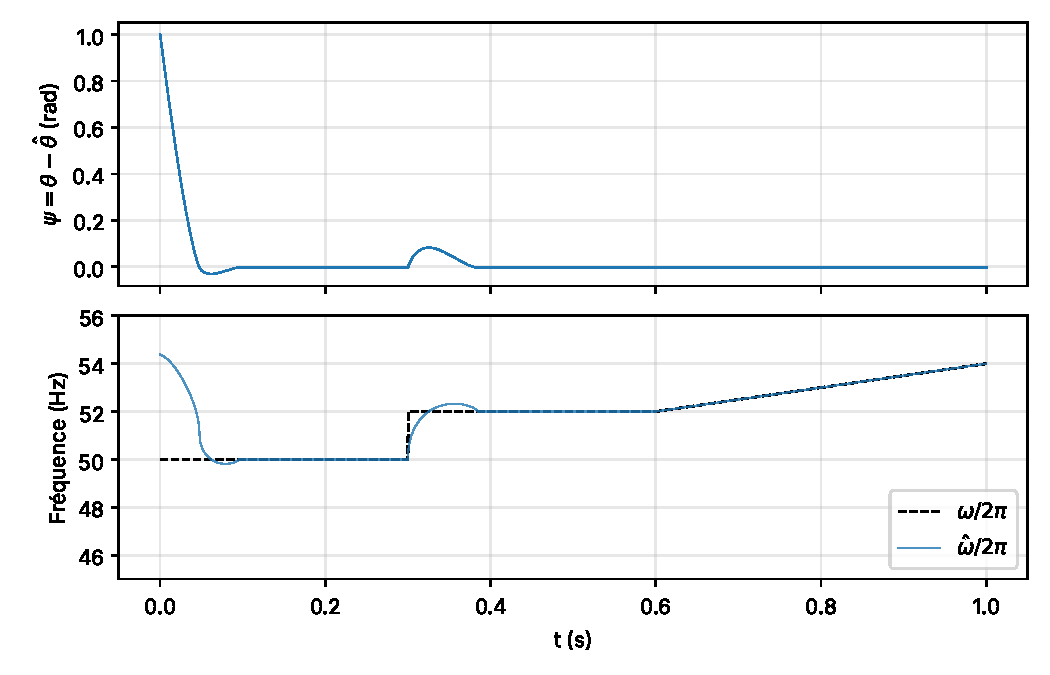
\includegraphics[width=0.85\textwidth]{figures/sim_pll_sta.pdf}
\caption{$\psi(0)=1$ rad, saut de fréquence de $+2$ Hz à $t=0.3$ s, puis rampe de 5 Hz/s
à partir de $t=0.6$ s ($k_1=30$, $k_2=150$).}
\end{figure}

%=====================================================================
\section{Implémentation numérique}
%=====================================================================

Avec une période d'échantillonnage $T_s$ et la méthode d'Euler, au pas $n$ :
\begin{enumerate}
  \item Mesurer $V_a[n],V_b[n],V_c[n]$.
  \item Clarke : $V_\alpha = \frac23(V_a-\frac12V_b-\frac12V_c)$, \quad $V_\beta = \frac{1}{\sqrt3}(V_b-V_c)$.
  \item Amplitude : $\hat V_m = \sqrt{V_\alpha^2+V_\beta^2}$ (on la protège contre la division par zéro).
  \item Erreur : $e = \big(-V_\alpha\sin\hth[n]+V_\beta\cos\hth[n]\big)/\hat V_m$.
  \item Fréquence : $\hw[n] = k_1\sqrt{|e|}\,\sign(e) + z[n] + \wff$.
  \item Intégrateur : $z[n+1] = z[n] + T_s\,k_2\sign(e)$.
  \item Angle : $\hth[n+1] = \big(\hth[n] + T_s\,\hw[n]\big)\bmod 2\pi$.
\end{enumerate}

%=====================================================================
\section{Limites de l'analyse}
%=====================================================================
\begin{itemize}
  \item \textbf{Saut de fréquence.} Il viole l'hypothèse \ref{H2}, mais se traduit simplement par
        un saut de $x_2$. La convergence reste garantie si le nouvel état est dans $\Omega$.
  \item \textbf{Déséquilibre et harmoniques.} La séquence inverse ajoute à $e$ une oscillation à $2\omega$.
        On n'a plus qu'une stabilité \emph{pratique} : $\psi$ reste dans un voisinage borné de 0.
        Un pré-filtrage (DSOGI, MAF) est recommandé.
  \item \textbf{Échantillonnage.} Le Super-Twisting discrétisé a une précision $|\psi|=O(T_s^2)$
        et $|x_2|=O(T_s)$ (Levant). Il faut y ajouter le retard d'un échantillon, $\approx\omega T_s$.
  \item \textbf{Sans normalisation.} Si l'on utilise $\varepsilon$ au lieu de $e$, le gain effectif devient
        $k_1\sqrt{V_m}$ (et $k_2$ ne change pas, car $\sign(\varepsilon)=\sign(e)$). La condition
        \eqref{eq:k2cond} doit alors être vérifiée pour le plus petit $V_m$ prévu.
\end{itemize}

%=====================================================================
\section{Corrections par rapport au tableau}
%=====================================================================
\begin{center}
\renewcommand{\arraystretch}{1.35}
\begin{tabular}{|p{4.2cm}|p{4.6cm}|p{5.2cm}|}
\hline
\textbf{Au tableau} & \textbf{Correction} & \textbf{Raison}\\
\hline
$V_a = V_m\sin\theta$ et $V_\alpha=V_m\cos\theta$ & choisir $V_a=V_m\cos\theta$ & sinon $V_\alpha=V_m\sin\theta$, $V_\beta=-V_m\cos\theta$ (section~\ref{sec:conv})\\
\hline
$\dot\varepsilon = V_m\cos\psi$ & $\dot\varepsilon = V_m\cos\psi\,\dot\psi$ & dérivation en chaîne (section~\ref{sec:edot})\\
\hline
$\dot V = V_m\cos\psi\sin\psi$ & $\dot V = V_m^2\sin\psi\cos\psi(\omega-\hw)$ & $\dot V=\varepsilon\dot\varepsilon$\\
\hline
$\hw = -k_1|\varepsilon|^{1/2}\sign\varepsilon + z$, $\dot z=-k_2\sign\varepsilon$ & signes $+$ & sinon divergence (section~\ref{sec:signe})\\
\hline
$\frac{d\theta}{dt}=\omega$ (encadré) & $\frac{d\hth}{dt}=\hw$ & c'est l'intégrateur de la PLL\\
\hline
$V=\frac12\varepsilon^2$ & $V=\zeta^\top P\zeta$ & une fonction quadratique en $\varepsilon$ ne prouve pas la convergence en temps fini du Super-Twisting\\
\hline
\end{tabular}
\end{center}

%=====================================================================
\appendix
\section{Annexe : rappels mathématiques}\label{sec:annexe}
%=====================================================================
\setcounter{equation}{0}
\renewcommand{\theequation}{A.\arabic{equation}}

\subsection*{Trigonométrie}
\begin{align}
\cos(a\pm b) &= \cos a\cos b\mp\sin a\sin b,\\
\sin(a\pm b) &= \sin a\cos b\pm\cos a\sin b .\label{A:sin}
\end{align}
En additionnant et en soustrayant les deux formes de $\cos(a\pm b)$ :
\begin{align}
\cos(a-b)+\cos(a+b) &= 2\cos a\cos b,\label{A:sum}\\
\cos(a-b)-\cos(a+b) &= 2\sin a\sin b .\label{A:diff}
\end{align}
Valeurs utiles :
\begin{equation}
\cos\tfrac{2\pi}{3} = -\tfrac12,\qquad \sin\tfrac{2\pi}{3} = \tfrac{\sqrt3}{2},\qquad \cos^2x+\sin^2x=1 .
\end{equation}

\subsection*{Fonction signe}
\begin{equation}
\sign(x) = \begin{cases}+1 & x>0\\0 & x=0\\-1&x<0\end{cases},\qquad x = |x|\sign(x),\qquad \sign(x)^2=1\ (x\neq0).
\end{equation}
Pour $x\neq0$, la dérivée de $|x|$ est $\sign(x)$, et $\sign$ est constante (dérivée nulle).

\subsection*{Dérivation}
\textbf{Dérivation en chaîne :} si $y=f(u(t))$, alors
\begin{equation}
\dot y = f'(u)\,\dot u .\label{A:chain}
\end{equation}
\textbf{Règle du produit :}
\begin{equation}
\frac{d}{dt}(uv) = \dot u\,v + u\,\dot v .\label{A:prod}
\end{equation}
\textbf{Dérivées partielles :} si $y=f(u(t),v(t))$,
\begin{equation}
\dot y = \frac{\partial f}{\partial u}\dot u + \frac{\partial f}{\partial v}\dot v .
\end{equation}

\subsection*{Matrices}
\textbf{Critère de Sylvester :} une matrice symétrique $2\times2$ $M$ est définie positive si et seulement si
\begin{equation}
M_{11}>0\ (\text{ou } M_{22}>0)\quad\text{et}\quad \det M>0 .\label{A:syl}
\end{equation}
\textbf{Inégalité de Rayleigh :} pour $M$ symétrique,
\begin{equation}
\lambda_{\min}(M)\|x\|^2\le x^\top Mx\le\lambda_{\max}(M)\|x\|^2 .\label{A:ray}
\end{equation}
\textbf{Transposée d'un produit :} $(AB)^\top = B^\top A^\top$, donc $(PA)^\top = A^\top P$ si $P=P^\top$.

\begin{thebibliography}{9}
\bibitem{moreno08} J.~A.~Moreno, M.~Osorio, \og A Lyapunov approach to second-order sliding mode
controllers and observers\fg, \emph{IEEE Conference on Decision and Control}, 2008.
\bibitem{moreno12} J.~A.~Moreno, M.~Osorio, \og Strict Lyapunov functions for the super-twisting
algorithm\fg, \emph{IEEE Transactions on Automatic Control}, 57(4):1035--1040, 2012.
\bibitem{levant93} A.~Levant, \og Sliding order and sliding accuracy in sliding mode control\fg,
\emph{International Journal of Control}, 58(6):1247--1263, 1993.
\bibitem{khalil} H.~K.~Khalil, \emph{Nonlinear Systems}, 3\textsuperscript{e} éd., Prentice Hall, 2002.
\end{thebibliography}

\end{document}
